\section{Анализ предметной области}
\subsection{Принцип работы программно-информационной системы управления бизнесом}

Согласно федеральному закону «О применении контрольно-кассовой техники при осуществлении расчетов в Российской Федерации» практически все заведения общественного питания должны быть оборудованы кассовым аппаратом. Современные ККТ, при совершении расчетов, передают данные в налоговую службу, а также используют их для автоматизации бизнес процессов. Кассовая программа позволяет автоматизировать все рабочие процессы предприятия. Рассмотрим, основные из них:

\subsubsection{Обслуживание гостей}
После принятия заказа и внесения его в программу, он сразу же отправляется на кухонные и барные чековые принтеры. В чеках указывается название блюда, его количество, а также пожелания гостей касаемо их заказа. При расчете гость получает чек с перечнем заказанного, суммой оплаты, а также размером скидки, если она была используема. Помимо этого, кассовые программы упрощают управление системой лояльность. После проведения оплаты через кассу, данные передаются в налоговую службу.

\subsubsection{Кухня и бар}
Программно-информационные системы управления ресторанным бизнесом позволяют автоматизировать работу с технологическими картами, обеспечивая контроль не только за качеством приготовления пищи, но и использованием продуктов, ведения учёта остатков ингредиентов и готовых блюд. Более того, система сама подсчитывает количество калорий, белков, жиров и углеводов как в объеме приготовленного, так и для каждой порции.
Автоматизация процессов для бара также, как и для кухни, позволяет создавать и управлять техническими картами. Стоит отметить, что согласно Федеральному закону №171, при работе бара с алкогольными напитками система обязана передавать данные в ЕГАИС с помощью универсального транспортного модуля.


\subsubsection{Бухгалтерия}
Программы для оптимизации ресторанного бизнеса могу интегрироваться с сервисами для бухгалтерского учета, например, 1С или Контур.экстерн или Отчет.ру. Благодаря этому взаимодействию, накладные и данные о продажах автоматически отправляются бухгалтерам, за счет чего минимизируются ошибки и сокращается время ожидание документа. Главной целью, интеграции является оптимизация закупок, работы с поставщиками и расчета остатков.

\subsubsection{Управление прибылью}
Для управления прибылью в системе используется раздел «Аналитика», с помощью которого отслеживается эффективность работы сотрудников, производительность предприятия. Анализируются данные о продажах блюд, выручку, прибыль, рентабельность. На основе этой статистики, владельцы заведений общественного питания, могут изменять меню, проводить работы с сотрудниками, следить за развитием своего предприятия. 

\subsubsection{Сотрудники} 
Для удобства работы с сотрудниками, в системах автоматизации существует модуль управления работниками заведения. Он позволяет сохранять данные персонала в базу, отслеживать количество перерывов и выходных, отработанных часов и смен.


\subsection{Компоненты программно-информационной системы управления ресторанным бизнесом}
Программно-информационная система управления ресторанным бизнесом представляет собой комплекс взаимодействующих программ, аппаратных средств и методов, предназначенных для хранения, обработки и предоставления информации. Важным условием функционирования данной системы является наличие выделенной точки доступа WI-FI, которая обеспечивает взаимодействие между различными модулями. Для предотвращения несанкционированного доступа и обеспечения безопасности данных, сеть WI-FI должна быть защищена паролем и иметь свой уникальный идентификатор (SSID). 
На рисунке ~\ref{system:image} представлена схема взаимодействия программных продуктов, входящих в систему управления ресторанным бизнесом, а также способы их взаимодействия.

\begin{figure}[ht]
	\centering
	\includegraphics[width=1\linewidth]{system} 
	\caption{Схема взаимодействия компонентов системы управления ресторанным бизнесом}
	\label{system:image}
\end{figure}


\subsection{Кассовые отчёты}
Одной из причин использования кассовых программ в заведениях общественного питания является удобство формирования отчётов. В большинстве касс есть раздел "<Отчёты">, в котором представлена статистическая документация для таких категорий как касса, выручка, расход блюд, специальные отчёты. Рассмотрим обязательные отчёты: 

\subsubsection{Z-отчёт}
Буквой Z обозначается отчёт о закрытии смены. Он представляет собой документ, фиксирующий финансовые итоги деятельности кассовой техники за определенный период времени. Z-отчёт формирует данные денежных счетчиков на момент начала и окончания смены, данные об общей выручке до обнуления, сведения о предоставленных скидках, аннулированных чеках, а также информация о произведенных возвратах. Пример отчета представлен на рисунке ~\ref{zotchet:image}.

\begin{figure}[ht]
	\centering
	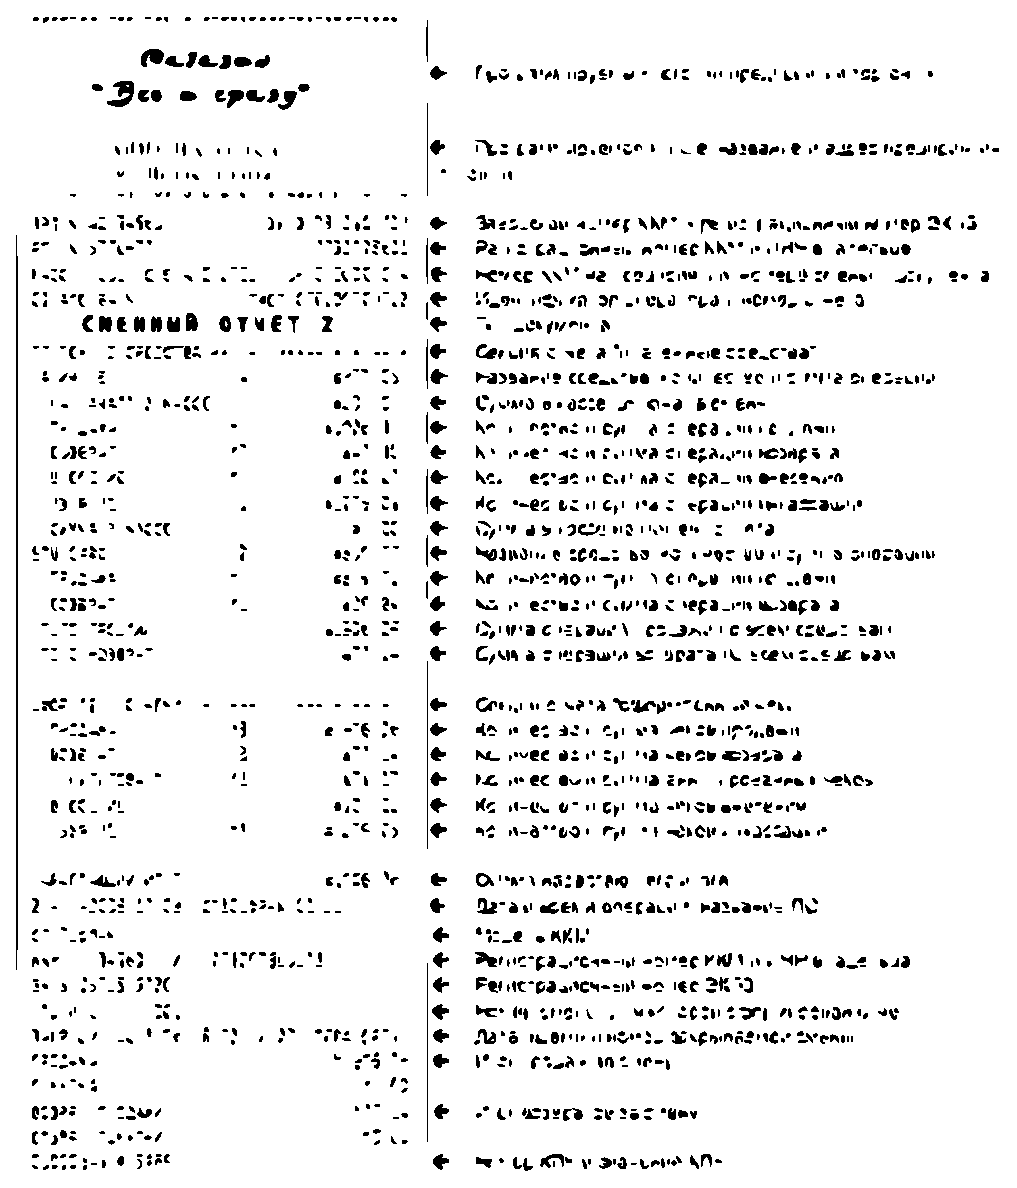
\includegraphics[width=0.7\linewidth]{zotchet} 
	\caption{Формат Z-отчёта}
	\label{zotchet:image}
\end{figure}

Ключевой особенностью данного отчёта является строго регламентированный временной интервал между двумя последовательными Z-отчётами, который не должен превышать 24 часа. Нарушение этого требования влечёт за собой блокировку кассового аппарата. Кроме того, каждому отчёту присваивается уникальный порядковый номер, исключающий возможность возникновения временных пробелов при формировании отчётности за определенный период времени.  

Поскольку в большинстве кассовых систем информация о закрытии смены фиксируется не только в контрольной ленте, но и в фискальной памяти устройства, Z-отчёт не подлежит обнулению и повторному формированию.  

В процессе обязательной регистрации контрольно-кассовой техники первоначальный Z-отчёт формируется и сохраняется в Инспекции Федеральной налоговой службы (ИФНС). Последующее формирование отчётов о закрытии смены приводит к обнулению оперативных данных о финансовой деятельности заведения за текущий день, а необходимые сведения автоматически передаются в налоговую. 

Z-отчёт необходим: 

\begin{itemize}
	\item кассиру для закрытия смены и передачи выручки в бухгалтерию: 
	\item бухгалтеру для контроля ежедневной выручки; 
	\item собственнику для анализа эффективности бизнеса; 
	\item сотрудникам налоговой для проверки правильности начисления и уплаты налогов. 
\end{itemize}

Содержание Z-отчёта должно соответствовать приказу ФНС России от 14.09.2020 № ЕД‑7‑20/662@. Перечень обязательных реквизитов представлена в Таблице \ref{zotchet:table}.

\begin{xltabular}{\textwidth}{|>{\raggedright\arraybackslash}p{5cm}|X|X|} 
	\caption{Обязательные данные для составления Z-отчёта\label{zotchet:table}} \\ \hline
	Наименование реквизита  & \centrow  Формат & \centrow Хранение \\ \hline
	\endfirsthead
	\continuecaption{Продолжение таблицы \ref{zotchet:table}}
	Наименование реквизита & \centrow Формат & \centrow Хранение \\ \hline 
	\finishhead
	Наименование документа& Печатный & - \\ \hline 
	Код формы ФД& Электронный & 5 лет \\ \hline
	Номер версии ФФД& Электронный &30 дней \\ \hline
	Наименование пользователя& Печатный & - \\ \hline
	ИНН пользователя & Печатный \newline Электронный & - \\ \hline
	Кассир& Печатный \newline Электронный & 30 дней \\ \hline 
	ИНН кассира& Печатный \newline Электронный & 30 дней \\ \hline
	Адрес расчётов& Печатный \newline Электронный & - \\ \hline
	Место расчётов& Печатный \newline Электронный & - \\ \hline
	Дата, время формирование документа& Печатный \newline Электронный & 5 лет \\ \hline
	Номер смены& Печатный \newline Электронный & 5 лет \\ \hline
	Регистрационный номер ККТ& Печатный \newline Электронный & 30 дней \\ \hline
	Количество кассовых чеков за смену& Печатный \newline Электронный & 30 дней \\ \hline
	Общее количество ФД за смену& Печатный \newline Электронный & 30 дней \\ \hline
	Количество непереданных ФД& Печатный \newline Электронный & 30 дней \\ \hline
	Дата первого непереданного ФД& Печатный \newline Электронный & 30 дней \\ \hline
	Признак превышения времени ожидания ответа ОФД& Печатный \newline Электронный & 30 дней \\ \hline
	Ресурс ключей фискального признака& Печатный \newline Электронный & 30 дней \\ \hline
	Номер фискального документа& Печатный \newline Электронный & 5 лет \\ \hline
	Номер фискального накопителя& Печатный \newline Электронный & 5 лет \\ \hline
	Фискальный признак документа& Печатный \newline Электронный & 5 лет \\ \hline
	Фискальный признак сообщения& Электронный & 30 дней \\ \hline
\end{xltabular} 
 
\subsubsection{X-отчёт}
Буквой X обозначают отчёт о текущем состоянии смен. Он представляет собой не фискальный документ, формируемый контрольно-кассовой техникой в течение открытой смены, так как информация, необходимая для формирования X-отчёта храниться в оперативной памяти ККТ и автоматически стирается, после закрытия смены.

В отличии от Z-отчёта X-отчёт не является документом строгой отчётности, передаваемым в налоговые органы, следовательно, он может быть сформирован неограниченное количество раз за одну смену. 

Предназначение X-отчёта заключается в предоставлении информации о текущем состоянии смены, денежных регистров и движении денежных средств в кассовом аппарате. Этот отчёт необходим собственнику бизнеса для внутреннего контроля и сверки данных о продажах, проходящих через контрольно-кассовую технику. 

Пример x-отчета можно увидеть на рисунке ~\ref{zotchet:image}. Его структура не определена законодательными требованиями. Она зависит от выбранного программного обеспечения кассового устройства. Однако, любой x-отчёт содержит следующие ключевые параметры: 

\begin{itemize}
	\item дата и время формирования отчёт; 
	\item сумма наличных денежных средств в кассе на момент формирования отчёта; 
	\item общий итог продаж за текущую смену; 
	\item количество и суммы оплат наличным и безналичным способами; 
	\item общее количество чеков за смену; 
	\item информацию о количестве и сумме возвратов. 
\end{itemize}

\begin{figure}[ht]
	\centering
	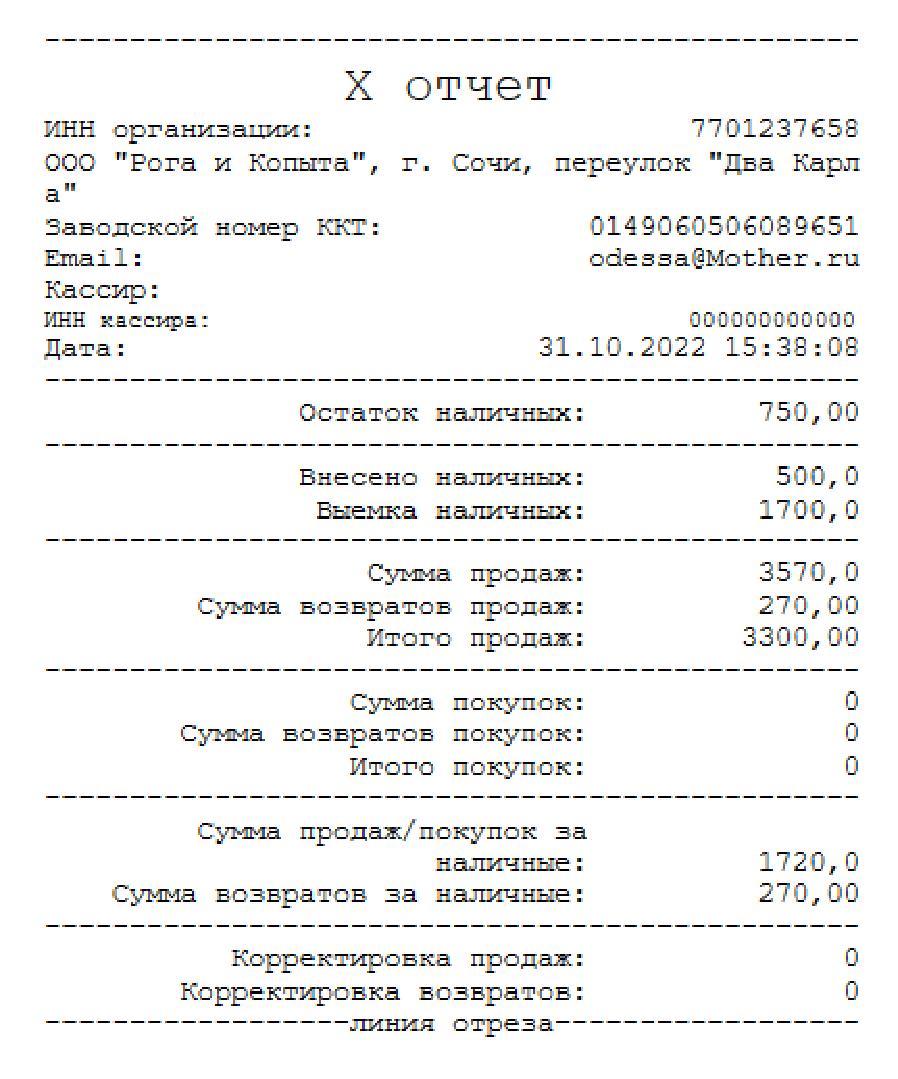
\includegraphics[width=0.5\linewidth]{xotchet} 
	\caption{Формат X-отчёта}
	\label{xotchet:image}
\end{figure}
